\documentclass[pdflatex,sn-basic,Numbered]{sn-jnl}
\usepackage{amsmath,amssymb,graphicx,booktabs,placeins,flafter,url,longtable,seqsplit}
% Use standard floats: the automatic threeparttable wrapper conflicts with resizebox.
\let\table\tableorg
\let\endtable\endtableorg
\newcommand{\toolace}{ToolACE}
\newcommand{\retool}{ReTool}
\newcommand{\glaive}{Glaive-FC}
\begin{document}
\title{Training on Broken Contexts: Source Loss and Repair in Tool-Augmented LLM Post-Training}
\author*[1]{\fnm{Amir Reza} \sur{Peimani}}
\email{amir.peimani@utoronto.ca}
\affil*[1]{\orgdiv{Institute of Biomedical Engineering},
\orgname{University of Toronto},
\orgaddress{\city{Toronto}, \country{Canada}}}
\abstract{Tool-augmented supervised fine-tuning can keep assistant targets in the training loss after sequence construction has separated them from the tool observations that supplied their values. We audit this failure by tracking each rendered token back to its original conversation and testing whether matched tool observations remain visible after assistant masking, truncation, splitting, and packing. We analyze ToolACE, ReTool, and a 5,000-conversation sample of Glaive-FC across six token budgets and several sequence-construction policies. At 512 tokens, BFD-split separates 38.66\%, 19.61\%, and 6.43\% of retained matched targets from their recorded sources in ToolACE, ReTool, and Glaive-FC, affecting 2.67\%, 15.05\%, and 8.60\% of conversations. Default BFD produces no such cases among retained matched targets, but retains only 17.23\% and 8.10\% of the original assistant supervision in ToolACE and ReTool. We then reconstruct training examples so that complete targets remain with the tool observations they use. On ToolACE at 512 tokens, grouping targets from the same conversation retains 875/918 matched targets while reducing the retained input-token ratio from 0.325 to 0.275 and eliminating 1,244 duplicated source tokens compared with reconstructing one example per target. For tool-call supervision, reducing the retained schema to the referenced parameters increases ToolACE coverage from 28.60\% to 73.15\%. Implementation checks also uncover a multi-batch token-stream defect in TRL 1.9.2 wrapped packing. Sequence construction therefore affects both how much supervision reaches the optimizer and whether that supervision is paired with the context that produced it.}
\keywords{{LLM post-training, supervised fine-tuning, tool-using agents, sequence packing, training data, data auditing}}
\maketitle

\section{Introduction}

Tool-using language models are commonly fine-tuned on trajectories containing user requests, tool calls, tool observations, and assistant responses. The stored conversation, however, is not the object presented to the optimizer. A chat template converts messages into tokens, an assistant mask selects the tokens that contribute to the loss, and sequence-construction code truncates, splits, or packs the result to fit a fixed context length. These operations can leave an assistant answer in the loss after placing the tool observation that supplied part of that answer outside its attention group.

Consider a tool that returns an order identifier, inventory location, measurement, or error code, followed by an assistant response that uses the returned value. If sequence construction separates the observation from the answer, the answer tokens can still be optimized even though the recorded value is no longer present in their context. Counting retained sequences or loss tokens does not expose this case because the supervision itself has survived.

Existing work on sequence construction has largely focused on efficient context use, arbitrary truncation, batching, and interactions between examples packed into the same sequence. Best-fit packing reduces document truncation \citep{ding2024fewer}, LongAlign and hierarchical balance packing address long-context data construction and batching \citep{bai2024longalign,yao2025hbp}, and recent SFT studies examine cross-example context effects and the conditions under which packing improves training \citep{dong2024tfp,wang2024packing}. Tool-use trajectories add a different dependency: later supervised tokens may rely on specific observations, user constraints, or tool declarations earlier in the trajectory.

Recent agent-training work makes some of these dependencies explicit before fine-tuning. Graph Explorer executes knowledge-graph trajectories under the deployed context rules and retains action supervision only when the identifiers used by an action are visible at that point \citep{chen2026graphexplorer}. ACC recompiles agent trajectories so that observations collected across tool turns become direct long-context supervision \citep{su2026acc}, while WebClipper prunes trajectory structure before training \citep{wang2026webclipper}. Our question arises after these higher-level trajectory decisions have been made: once a conversation has been rendered, masked, truncated, split, and packed, does a supervised target still contain the recorded context from which it was produced?

We answer this question by tracking the origin of every token through sequence construction. For values that can be matched directly from a tool observation to the following assistant response, we test whether the original observation remains earlier in the same attention group as the supervised target. We report the fraction of matched targets that lose their source, the fraction of conversations affected, and the fraction of the original assistant objective contributed by the affected target tokens.

Across ToolACE, ReTool, and Glaive-FC, sequence policies that split conversations across training examples frequently retain targets after separating them from their recorded tool observations. At a 512-token budget, BFD-split affects 38.66\% of retained matched targets in ToolACE, 19.61\% in ReTool, and 6.43\% in Glaive-FC. These cases occur in 2.67\%, 15.05\%, and 8.60\% of conversations, respectively. Default BFD produces no such separations among retained matched targets in these audits, but retains only 17.23\% of the original assistant supervision in ToolACE and 8.10\% in ReTool. The choice of sequence policy therefore changes both supervision retention and the context available to that supervision.

We also reconstruct shorter training examples that keep complete targets with the matched tool observations they use. Combining compatible targets from the same conversation reduces repeated context without reducing target coverage. On ToolACE at 512 tokens, grouping retains 875/918 matched targets, the same number as reconstructing a separate example for each target, while reducing the retained input-token ratio from 0.325 to 0.275 and eliminating 1,244 duplicated source tokens. For tool-call targets, large tool schemas create a second context-length problem. Keeping only the invoked tool or the parameters used in the call raises short-budget coverage substantially on ToolACE, whereas ReTool's compact schemas are better kept intact.

Finally, we test the sequence-construction implementations themselves against token-level fixtures. These tests uncover a multi-batch defect in the TRL 1.9.2 wrapped-packing path that changes the emitted token stream at Arrow map boundaries. This result is analyzed separately from the packing-policy comparison,
which uses the single-batch implementation of the intended concatenate-then-split operation.

The paper makes three main contributions:
\begin{enumerate}
    \item We develop a token-level audit that tests whether supervised targets in tool-augmented SFT still have access to the tool observations from which their matched values were obtained after rendering and sequence construction.

    \item We measure this failure across three released tool-training corpora, six token budgets, and multiple packing and truncation policies, showing large differences across datasets and a clear interaction between target context and supervision retention.

    \item We reconstruct training examples to retain matched observation-to-answer and user-to-tool-call relations under fixed token budgets. Grouping reduces duplicated context at unchanged target coverage, and reducing large tool schemas substantially increases short-context tool-call coverage.
\end{enumerate}

\section{Related Work}

\paragraph{Training trajectories for tool-using agents.}
Tool-use trajectories contain dependencies between user requests, tool calls, tool observations,
and later actions or answers. Recent work has increasingly used these dependencies when generating
or filtering training data. Graph Explorer executes knowledge-graph trajectories under the same
context rules used by the agent and retains action supervision only when the identifiers required
by the action remain visible \citep{chen2026graphexplorer}. Anchor generates GUI-agent trajectories
from verified branch points and filters actions using state-based checks
\citep{wei2026anchor}. WebClipper removes redundant and inefficient branches from web-agent
trajectories \citep{wang2026webclipper}, while ACC recompiles multi-turn agent trajectories into
long-context question--answer training examples \citep{su2026acc}. TRACER links generated claims
to the tool observations used to produce them \citep{yu2026tracer}.

These methods operate during trajectory generation, filtering, or restructuring. We begin with an
existing tool-use trajectory and examine what happens afterward, when chat rendering, masking,
truncation, splitting, and packing produce the token sequences used for supervised fine-tuning.

\paragraph{Sequence construction and packing.}
Sequence construction affects both training efficiency and the context presented to the model.
Best-fit packing reduces arbitrary document truncation \citep{ding2024fewer}, while LongAlign and
hierarchical balance packing address batching and data construction for long-context training
\citep{bai2024longalign,yao2025hbp}. For supervised fine-tuning, Threshold Filtering Packing groups
related examples within packs \citep{dong2024tfp}, and Packing Analysis studies when packing
improves efficiency without degrading downstream performance \citep{wang2024packing}.

We examine a different consequence of sequence construction within tool-use trajectories. A target
can remain in the training loss after the tool observation containing its value has been placed in
a different attention group. We measure this after the complete rendering, masking, and
length-handling procedure, rather than from the stored conversation or its nominal length.

\paragraph{Tool-use training data and tool observations.}
ReAct established the widely used reason--act--observe interaction pattern
\citep{yao2023react}, and ToolLLM, ToolACE, and ReTool developed large-scale training methods and
datasets for tool use and function calling
\citep{qin2024toolllm,liu2025toolace,feng2025retool}. Data quality is consequential in this
setting: filtering synthetic tool-use examples for correctness can improve downstream tool
performance even with fewer training examples \citep{iskander2024quality}. Models can also fail
to extract and use information from tool outputs even when those outputs are present in the
inference context \citep{kate2026tooloutputs}.

Our analysis addresses the preceding training-data problem. Before asking whether a model learns
to use a tool observation correctly, we test whether the observation is still present when the
corresponding answer tokens are optimized.


\section{Audit Definition}
\label{sec:formulation}

A stored conversation is rendered with the model's chat template and assistant loss mask and is
then truncated, split, or packed into training sequences. We record the original conversation and
rendered-token position of every output token throughout these operations. This allows a value in
an assistant target to be traced back to the particular tool observation from which it was
matched, even when the same string occurs elsewhere.

The primary analysis considers values copied from a tool observation into the immediately following
assistant message. A value is included when it can be located in both messages after full chat
rendering and has not already appeared in earlier non-tool text. Details of value extraction and
matching are given in Section~\ref{sec:relation_extraction}.

After sequence construction, a matched target is retained if its target-value tokens still
contribute to the training loss. Its recorded tool value remains available if the complete matched
occurrence appears earlier in the same attention group as the supervised target-value tokens.
An identical value from another conversation or another position does not count as the recorded
source.

We count a retained target as \emph{separated} when its matched tool value is no
longer available under the final attention structure. If several matched values connect
the same tool observation and assistant message, they are treated as one target unit,
and the target is counted as separated if any of those values loses its recorded source.

We report three quantities. The separation rate is the fraction of retained matched
targets that are separated from their recorded tool values. We also report the fraction
of original conversations containing at least one separated target and the affected
target-value tokens as a fraction of the original assistant loss tokens. These quantities
measure the rate within the matched subset, its distribution across conversations, and
its contribution to the full SFT loss.

The primary analysis covers direct copied values. Paraphrases, calculations, multi-step semantic
dependencies, and other relations that cannot be tied to a specific occurrence in the recorded
trajectory are not included. A separate tool-call analysis matches quoted or numeric user
constraints to the following assistant tool call and includes the corresponding tool declaration
when evaluating context-length constraints.

\section{Methods}

\subsection{Matching tool values to assistant targets}
\label{sec:relation_extraction}

We identify direct observation-to-answer relations by matching values in tool observations to the immediately following assistant message. Candidate values are extracted from JSON leaves, fenced JSON, standalone numeric values, and plain stdout lines. A match is retained when the value appears in the following assistant message, has not appeared in earlier non-tool text, and both occurrences can be located after applying the full chat template.

Text matching is case-insensitive in the primary analysis, while numeric values are matched using lexical boundaries. We repeat the corpus analysis with strict case-sensitive matching. Prespecified subsets include nonnumeric values, values containing at least 6, 10, and 20 characters, and opaque structured codes. Paraphrases, calculations, and other semantic transformations are not included.

For tool-call targets, we separately match quoted or numeric constraints in the user message to values copied into the following assistant tool call. We then evaluate three amounts of accompanying schema context: the full schema block, the complete declaration of the invoked tool, and a valid schema containing only the referenced parameters and their associated metadata.


\subsection{Sequence construction policies}
\label{sec:policies}

We evaluate TRL 1.9.2 sequence construction at maximum lengths of 256, 512, 1,024, 2,048, 4,096, and 8,192 tokens. The evaluated policies are non-packed keep-start truncation, best-fit-decreasing (BFD) packing, BFD-split packing, wrapped packing, drop-overlength, and the deprecated keep-end truncation policy as a historical comparison \citep{trl2026,huggingface2026sft}.

BFD packs sequences using best-fit decreasing and truncates tokens beyond the maximum sequence length. BFD-split first divides overlength sequences into fragments no longer than the token budget and then packs those fragments. Wrapped packing concatenates tokenized examples into a continuous stream and divides the stream into fixed-length blocks, so a block boundary may fall inside an original conversation. TRL uses BFD as its default packing strategy and exposes BFD-split and wrapped as alternatives \citep{huggingface2026sft}. Its paper index provides a BFD-split configuration associated with the best-fit packing method of \citet{ding2024fewer}, and a public LongAlign regression script uses wrapped packing \citep{huggingface2026paperindex,diro2026wrapped}.

The analysis uses the causal sequence boundaries produced by each policy. For BFD and BFD-split, TRL emits \texttt{seq\_lengths} describing the sequences or fragments contained within each packed row. Under the padding-free execution evaluated here, position IDs restart at these boundaries, so each fragment is treated as a separate causal sequence. A target can therefore use only earlier tokens within its own fragment. Wrapped packing does not emit corresponding fragment boundaries; each wrapped block is treated as one causal sequence.


\subsection{Token tracking and implementation checks}
\label{sec:conformance}

For every token produced by sequence construction, we retain its original dataset row and position in the rendered conversation. We propagate the same information for loss labels. This lets us determine whether a target still contains the particular tool-value occurrence to which it was matched, rather than another occurrence of the same string.

We test our implementation against TRL using fixed synthetic examples. For each sequence policy, we compare the emitted token IDs, labels, packed boundaries, and \texttt{seq\_lengths} with TRL outputs. We also compare the rendered source and target spans with token IDs produced directly by \texttt{apply\_chat\_template}.

Wrapped packing is tested both with the released TRL 1.9.2 implementation and with a single-batch implementation of the intended concatenate-then-split operation. The policy comparisons use the single-batch token stream; the difference found in the released multi-batch implementation is reported separately in Section~\ref{sec:wrapped_defect}.


\subsection{Datasets and statistical analysis}
\label{sec:datasets}

We analyze the complete pinned releases of ToolACE and ReTool, containing 11,300 and 2,000 conversations, respectively. For Glaive-FC, we analyze 5,000 conversations selected from 39,591 examples satisfying the required multi-turn action--observation--answer structure in the Apache-2.0 release. Eligible conversations are ranked by SHA-256 hash, and the 5,000 lowest-ranked examples are retained. Dataset revisions, hashes, and the complete Glaive eligibility rule are reported in the appendix.

The observation-to-answer matcher yields 918 target units in ToolACE and 1,611 in ReTool. The Glaive-FC sample contains 6,713 target units at 512 tokens before policy-specific target loss. When several matched values connect the same tool observation and assistant message, they are treated as one target unit.

We report exact counts and percentages. For corpus-level proportions, 95\% confidence intervals are obtained from 2,000 cluster-bootstrap replicates \citep{efron1994bootstrap}. Each replicate resamples complete conversations with replacement and recomputes the statistic, keeping values from the same conversation together.


\subsection{Training-example reconstruction}
\label{sec:materialization}

We reconstruct shorter training examples containing complete assistant targets and the matched
tool observations used by those targets. For each target, the required content includes the
complete target message, the matched value occurrences in its tool observations, and the
chat-template tokens needed to serialize those source messages. After the required content has
been selected, any remaining token budget is filled with complete message blocks from the same
conversation, scanning backward from the latest selected target.

Targets from the same conversation are grouped when their combined required content fits within
the token budget. The grouping procedure is deterministic. Each group begins with the remaining
target requiring the largest number of tokens. Additional targets are then added in order of
smallest marginal token cost while they fit within the budget, with ties broken by their position
in the conversation. A new group is started when no remaining target fits.

Selected target messages are retained completely, tokens outside those targets receive label
$-100$, and each matched tool value must occur before the corresponding supervised target tokens
in the same causal sequence. Tokens from different original conversations are never combined.
Each serialized example is checked again after tokenization using the same token tracking and
visibility test as the corpus analysis.

We compare grouping with two alternatives. The first constructs one training example for each matched target. The second retains the complete tool-observation and assistant-response rounds associated with the target. We compare the number of matched targets retained, assistant target tokens retained, input tokens relative to the original rendered corpus, examples generated per source conversation, duplicated source tokens, sequence lengths, and changes in how often individual conversations appear in the reconstructed dataset.


\subsection{Tool-call schema reduction}
\label{sec:schema_repair}

For each matched user-constraint-to-tool-call relation, we construct an example containing the relevant user constraint, the complete assistant tool call, and one of three forms of tool schema.

The \emph{whole-schema} condition retains every tool declaration supplied with the conversation. The \emph{invoked-tool} condition retains only the complete declaration of the function called by the assistant. The \emph{parameter-slice} condition retains the invoked function and the descriptions, types, enums, defaults, constraints, and required status of the referenced parameters.

Calls with ambiguous function identity, missing declarations, or schemas that cannot be reconstructed as valid structures are not counted as covered. At each token budget, coverage is the fraction of matched tool-call targets that fit together with the relevant user constraint, complete tool call, and specified schema content.


\subsection{Controlled source-removal experiment}
\label{sec:controlled}

We also test whether removing tool values during training changes model behavior in a controlled exact-value task. The dataset contains six independently generated value families and 1,800 training examples. In separate training conditions, the tool observation containing the answer value is removed from 0\%, 25\%, 50\%, or 100\% of examples while the original assistant answer remains in the training loss.

We fine-tune Qwen2.5-0.5B-Instruct with LoRA \citep{yang2024qwen25,hu2022lora} using three optimization seeds. Evaluation uses held-out examples and measures exact target-value generation and target-value negative log-likelihood. The complete data-generation procedure, model configuration, evaluation sets, and family-level results are reported in the appendix.

\section{Results}

\subsection{Sequence splitting separates supervised targets from their tool observations}
\label{sec:source_loss_results}

\begin{figure}[t]
  \centering
  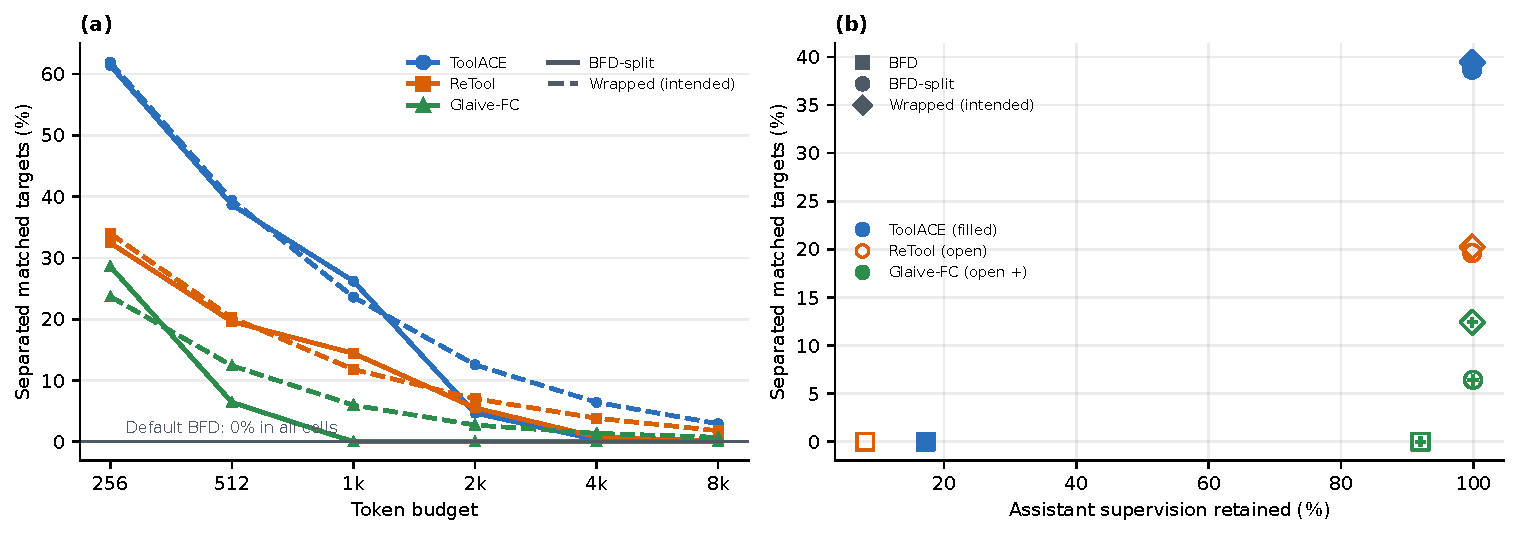
\includegraphics[width=\linewidth]{../figures/figure2_current_policy_incidence.pdf}
  \caption{
  Separation of matched assistant targets from their recorded tool observations across token budgets. (a) Fraction of retained matched targets whose tool value is no longer available after BFD-split or intended wrapped packing. Default BFD produces no such cases among retained matched targets in any corpus--budget combination. (b) Separation rate versus the fraction of original assistant supervision retained at 512 tokens
  }
  \label{fig:policy}
\end{figure}

At a 512-token budget, BFD-split separates 353/913 retained ToolACE targets from their matched
tool observations (38.66\%, 95\% cluster-bootstrap CI 35.50--41.98), 315/1,606 ReTool targets
(19.61\%, CI 17.74--21.76), and 431/6,698 Glaive-FC targets
(6.43\%, CI 5.87--7.04). The ToolACE rate remains similar in the prespecified
higher-specificity subsets: 297/773 nonnumeric targets (38.42\%), 171/417 values containing
at least 20 characters (41.01\%), and 46/134 opaque identifiers (34.33\%).

The rate falls as the token budget increases (Figure~\ref{fig:policy}a). The median contiguous
span needed to contain both the matched tool value and assistant target is 194 tokens for
ToolACE, 32 for ReTool, and 65 for Glaive-FC. The corresponding 95th percentiles are
913, 125, and 144 tokens.

Default BFD produces no target--source separations among the matched targets it retains, but
retains little assistant supervision on two of the three datasets. At 512 tokens, BFD retains
17.23\% of the original assistant loss tokens in ToolACE and 8.10\% in ReTool, compared with
91.99\% in Glaive-FC. BFD-split retains 99.79\%, 99.79\%, and 99.93\%, respectively
(Table~\ref{tab:primary}; Figure~\ref{fig:policy}b).

\begin{table}[t]
\centering
\small
\caption{
Primary comparison at a 512-token budget. ``Separated'' counts retained matched targets
whose recorded tool value is no longer available to the supervised target.
}
\label{tab:primary}
\begin{tabular}{llrrr}
\toprule
Corpus & Policy &
\shortstack{Matched targets\\retained} &
Separated &
\shortstack{Assistant supervision\\retained} \\
\midrule
ToolACE & BFD
& 10/918
& 0/10 (0.00\%)
& 17.23\% \\
& BFD-split
& 913/918
& 353/913 (38.66\%)
& 99.79\% \\
\addlinespace

ReTool & BFD
& 6/1,611
& 0/6 (0.00\%)
& 8.10\% \\
& BFD-split
& 1,606/1,611
& 315/1,606 (19.61\%)
& 99.79\% \\
\addlinespace

Glaive-FC & BFD
& 6,154/6,713
& 0/6,154 (0.00\%)
& 91.99\% \\
& BFD-split
& 6,698/6,713
& 431/6,698 (6.43\%)
& 99.93\% \\
\bottomrule
\end{tabular}
\end{table}

The corpus-wide impact differs substantially from the rate among matched targets. In ToolACE,
the 38.66\% target-level rate affects 302/11,300 conversations (2.67\%) and 2.089\% of the
original assistant loss tokens. In ReTool, 301/2,000 conversations are affected (15.05\%), but
the affected values contribute only 0.125\% of the original assistant loss because the matched
relations are dominated by short numeric values. Glaive-FC has 430/5,000 affected conversations
(8.60\%) and 1.224\% of assistant loss tokens affected.

Intended wrapped packing gives similar or higher rates at 512 tokens: 39.43\% in ToolACE,
20.24\% in ReTool, and 12.41\% in Glaive-FC. Strict case-sensitive matching changes the
estimates very little. Under BFD-split, the corresponding rates are 38.80\%, 19.84\%, and
6.58\%; under intended wrapped packing they are 39.62\%, 20.36\%, and 12.48\%. The largest
difference from the primary 512-token estimates is 0.22 percentage points. Results for all six
token budgets are reported in the appendix.


\subsection{Grouping retains the same targets with less duplicated context}
\label{sec:grouped_results}

\begin{figure}[t]
  \centering
  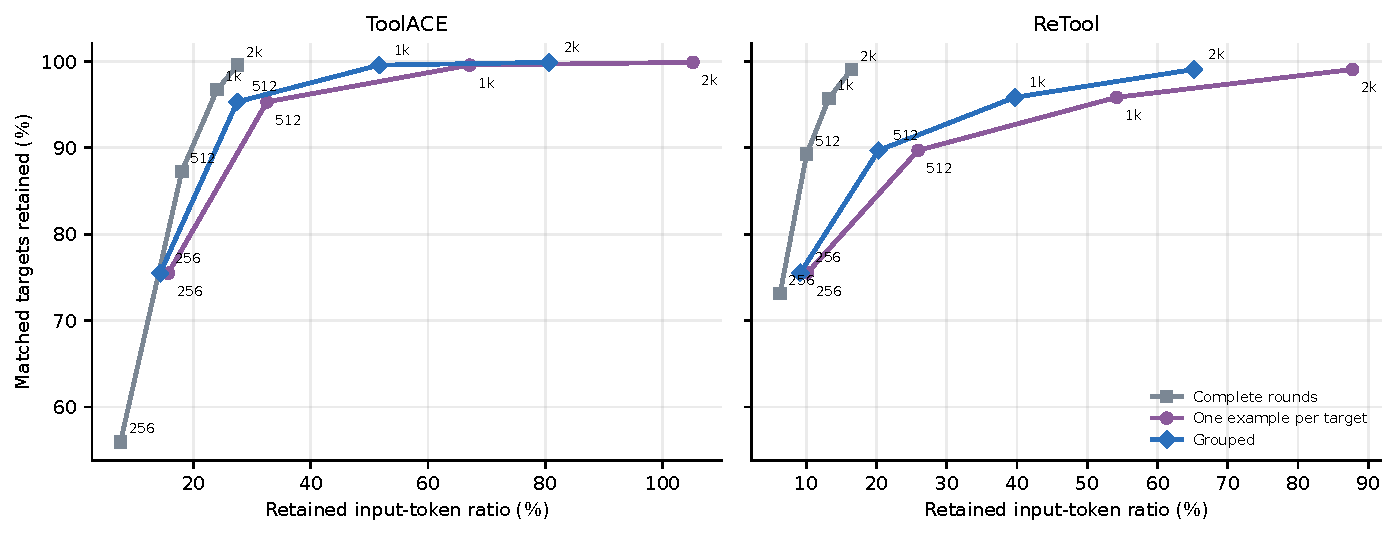
\includegraphics[width=\linewidth]{../figures/figure4_grouped_repair.pdf}
    \caption{
    Matched-target retention versus retained input-token ratio for (a) ToolACE and
    (b) ReTool at 256, 512, 1,024, and 2,048 tokens. Grouping targets from the same
    conversation generally matches one-example-per-target reconstruction using fewer input
    tokens. At 512 tokens, grouping reduces duplicated source tokens from 1,244 to zero in
    ToolACE and from 1,848 to 311 in ReTool
    }
  \label{fig:grouped}
\end{figure}

On ToolACE at 512 tokens, grouping and one-example-per-target reconstruction both retain
875/918 matched targets (95.32\%) and 82.19\% of target supervision. Grouping reduces the
retained input-token ratio from 0.325 to 0.275, reduces generated examples per original
conversation from 1.291 to 1.025, and eliminates all 1,244 duplicated source tokens.

Retaining the complete tool-observation and assistant-response rounds uses fewer input tokens,
with a ratio of 0.180, but retains only 801/918 targets (87.25\%) and 65.35\% of target
supervision. The difference is larger at short budgets. At 256 tokens, grouping retains
693/918 targets (75.49\%), compared with 514/918 (55.99\%) when complete rounds are kept.
At 1,024 tokens, grouping retains 914/918 targets (99.56\%).

ReTool shows the same advantage over one-example-per-target reconstruction. At 512 tokens, both
methods retain 1,445/1,611 matched targets (89.70\%). Grouping reduces the input-token ratio
from 0.259 to 0.203, examples per original conversation from 1.246 to 0.970, and duplicated
source tokens from 1,848 to 311. Figure~\ref{fig:grouped} shows the tradeoff between retained
targets and input tokens across budgets.


\subsection{Reducing large tool schemas increases short-context coverage}
\label{sec:schema_results}

\begin{figure}[t]
  \centering
  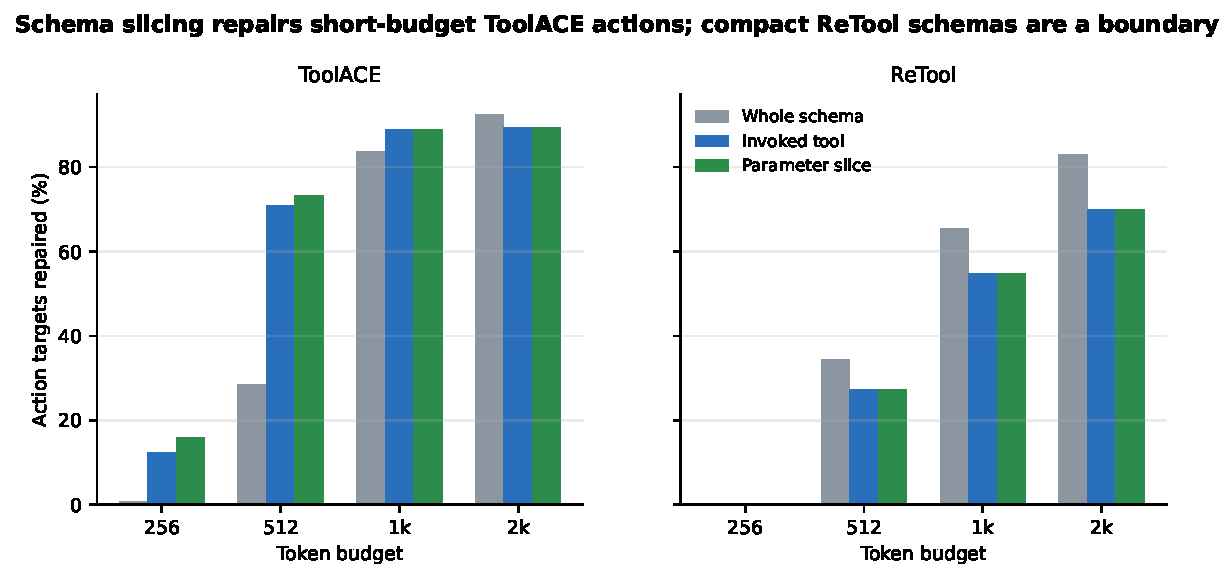
\includegraphics[width=\linewidth]{../figures/figure5_schema_repair.pdf}
  \caption{
  Fraction of matched tool-call targets that fit within the token budget together with the relevant user constraint, complete tool call, and specified schema content for (a) ToolACE and (b) ReTool. Reducing the schema substantially increases short-budget coverage in ToolACE, whereas ReTool's compact schemas are better retained in full
  }
  \label{fig:schema}
\end{figure}

Among 7,591 ToolACE tool-call targets, retaining the full schema allows 28.60\% to fit within
512 tokens. Retaining only the invoked tool increases coverage to 70.95\%, and retaining only
the referenced parameters increases it to 73.15\%. At 256 tokens, the corresponding rates are
0.67\%, 12.34\%, and 15.89\%. By 1,024 tokens, they rise to 83.70\%, 88.86\%, and 88.99\%.

ReTool shows the opposite ordering because its trajectories generally contain a compact
single-tool schema. At 512 tokens, the full schema fits with 34.42\% of targets, compared with
27.33\% for both reduced-schema variants. At 1,024 tokens, the corresponding rates are 65.44\%
and 54.80\%. The benefit of reducing schema content therefore depends mainly on how much of the
available token budget is occupied by tool declarations.


\subsection{TRL 1.9.2 wrapped packing changes the token stream across map batches}
\label{sec:wrapped_defect}

The released TRL 1.9.2 wrapped-packing implementation changes the intended token stream across
Arrow map batches. We constructed a 2,001-row fixture containing two unique tokens per row so
that every output position could be traced to its input row. The output matches the expected
stream through position 1,999 and first diverges at position 2,000, exactly at the default
1,000-row map boundary. Overall, 2,002/4,002 positions come from the wrong input location.
Processing the same fixture in a single map batch reproduces all 4,002 positions correctly.

Inspection of the implementation localizes the error to slice-local offsets being applied when
reconstructing arrays from unsliced \texttt{column.values}. This causes parts of earlier Arrow
storage to be repeated instead of preserving the intended concatenate-then-split stream.

The effect is also visible on ToolACE. At a 512-token budget, the released wrapped path contains
assistant-token occurrences equal to 296.3\% of the original assistant loss-token count, while unique coverage includes only 36.18\% of the original assistant loss-token positions
and 15.65\% of source-token positions. The single-batch implementation
of the intended wrapped operation retains 99.8\% of assistant supervision. All wrapped results
reported above therefore use that intended token stream.

\FloatBarrier

\section{Discussion}

Sequence construction changes the training signal in tool-augmented SFT. Across ToolACE, ReTool,
and Glaive-FC, BFD-split and wrapped packing frequently retain assistant targets after separating
them from the tool observations containing their matched values. At 512 tokens, this occurs for
38.66\% of retained matched targets in ToolACE, 19.61\% in ReTool, and 6.43\% in Glaive-FC.
The corpus-wide impact differs substantially across datasets. ToolACE has the highest target-level
rate but only 2.089\% of the original assistant loss tokens are affected. ReTool affects 15.05\%
of conversations but only 0.125\% of assistant loss tokens because most matched values are short
numeric fields. Reporting only one of these quantities would obscure an important part of the
result.

Default BFD shows the other side of the tradeoff. It produces no target--source separations among
the matched targets retained in our audits, but at 512 tokens it keeps only 17.23\% of the
original assistant supervision in ToolACE and 8.10\% in ReTool. BFD-split retains almost all
assistant supervision but separates some targets from their observations. Glaive-FC is less
affected because most matched observation--target spans fit within the available context.
Sequence construction therefore determines both the amount of supervision used for optimization
and the context attached to that supervision. This extends previous analyses of SFT packing,
which have focused primarily on efficiency, cross-example context effects, and downstream
performance \citep{wang2024packing}.

Grouping targets from the same conversation reduces the cost of reconstructing shorter examples.
On ToolACE, grouping retains the same 875/918 matched targets as creating one example per target,
while reducing the retained input-token ratio from 0.325 to 0.275 and eliminating 1,244 duplicated
source tokens. ReTool shows the same pattern. Repeated source context increases training tokens
and changes how often individual conversations appear in the reconstructed dataset, so combining
compatible targets is a more efficient way to retain the same supervision.

The tool-call experiments show that schema size can dominate the context budget. In ToolACE,
retaining the full schema allows only 28.60\% of matched tool-call targets to fit within 512
tokens, compared with 70.95\% when only the invoked tool is retained and 73.15\% when only the
referenced parameters are kept. ReTool behaves differently because its schemas are usually
compact and contain a single tool. The full declaration is therefore preferable in that dataset.
Schema reduction is useful when declarations are large enough to displace the user constraint
or tool call that the model is being trained to reproduce.

The TRL 1.9.2 wrapped-packing result shows that the implementation itself can alter the training
data beyond the intended packing rule. The released path first diverges from the expected token
stream exactly at the Arrow map-batch boundary and assigns 2,002/4,002 positions to the wrong
input locations in the controlled fixture. On ToolACE, the same behavior produces assistant-token
occurrences equal to 296.3\% of the original assistant loss-token count. Tracking the original row and position of each emitted token localizes the error to the
reconstruction of batched Arrow columns. The result shows why packing should be checked on the
emitted token stream instead of inferred from configuration settings.

The controlled source-removal experiment tests the learning consequence in a setting where the
tool value determines the answer. Removing the value from every training example reduces held-out
exact generation to zero and sharply increases target-value negative log-likelihood. Models trained
with 25\% or 50\% of examples missing the value still recover the held-out values in this task.
The experiment therefore shows that complete removal of the recorded tool information prevents
learning of the exact-value mapping, while partial corruption is tolerated at the tested scale.
The corpus analysis addresses a different question: how often real sequence-construction policies
produce such separations in released tool-training data.

Models already struggle to extract and use structured tool responses when those responses are
present in context \citep{kate2026tooloutputs}. Removing the corresponding observation during
training adds another failure before model reasoning becomes the limiting factor.

\paragraph{Limitations.}
The matcher covers values copied directly from a tool observation into the following assistant
message. Paraphrases, calculations, multi-step dependencies, and other semantic relations are not
counted. Some matched values may also be recoverable from other context or model knowledge. ToolACE, ReTool, and Glaive-FC contain generated tool-use trajectories, and Glaive-FC is
evaluated on a deterministic 5,000-conversation sample. Reconstructing shorter examples changes
some surrounding context and the frequency of examples derived from each conversation. The
controlled experiment uses one 0.5B model and a synthetic exact-value task.

\paragraph{Practical implications.}
Training code can retain the original conversation and rendered position of each token through
chat rendering, masking, truncation, splitting, and packing. These identifiers are sufficient to
check whether a matched tool value remains available when its answer tokens contribute to the
loss. Packing evaluations should report both assistant supervision retained and the fraction of
matched targets separated from their observations. When long trajectories must be split, grouping
compatible targets from the same conversation reduces repeated context, and large tool schemas can
be reduced to the invoked tool or referenced parameters when the full declaration consumes too
much of the token budget.


\section{Conclusion}

Tool-augmented SFT can retain assistant targets in the training loss after sequence construction
has separated them from the tool observations containing their values. We find this behavior
across three released tool-training corpora under policies that split conversations across training
sequences. Default BFD avoids the problem among retained matched targets, but at short token
budgets it discards most assistant supervision in ToolACE and ReTool.

Grouping targets from the same conversation retains the same supervision with fewer duplicated
tokens, and reducing large tool schemas substantially increases tool-call coverage at short context
lengths. We also identify a TRL 1.9.2 wrapped-packing defect that changes the emitted token stream
across map batches. Sequence construction is therefore part of the effective training data in
tool-augmented LLM fine-tuning and should be evaluated at the final token-sequence level.


\backmatter
\section*{Statements and Declarations}
\subsection*{Author contributions}
Amir Reza Peimani conceived the study, developed the methods, performed the
analyses, and wrote and revised the manuscript.
\subsection*{Funding}
No funding was received for conducting this study.
\subsection*{Competing interests}
The author has no relevant financial or non-financial interests to disclose.

\subsection*{Data and code availability}
The code, configurations, recorded results, and data acquisition instructions are available at
\url{https://github.com/AmirRezaPeimani/when-supervision-outlives-support}.
Dataset and model revisions, licenses, and reproduction details are provided in the appendix.
A snapshot of the reproducibility package used for this submission is provided as Online Resource~1.

\begin{appendices}
\setcounter{table}{1}
\setcounter{figure}{3}
\renewcommand{\thetable}{\arabic{table}}
\renewcommand{\thefigure}{\arabic{figure}}
\section{Reproducibility}

Online Resource~1 contains the code, configurations, and recorded outputs used for
conversation rendering, token tracking, sequence-policy evaluation, value matching,
training-example reconstruction, tool-call schema reduction, and the controlled model experiment.
Experiment records include dataset or model revisions, random seeds where applicable, raw outputs,
derived results, runtime, and compute information. The test suite covers chat-template rendering,
source and target span mapping, token tracking through packing, causal sequence boundaries,
training-example reconstruction, schema validity, TRL output checks, and
train/development/test separation.

The main reproduction commands are:

\begin{verbatim}
PYTHONPATH=src python scripts/run_phase1.py \
  --config configs/primary_audit.json \
  --output-dir outputs/raw/phase1_attention_corrected

PYTHONPATH=src python scripts/run_phase1_glaive.py \
  --config configs/glaive.json \
  --output-dir outputs/raw/glaive_attention_corrected

PYTHONPATH=src python scripts/run_phase1.py \
  --config configs/case_sensitive_toolace_retool.json \
  --output-dir outputs/raw/case_sensitive_tool_retool

PYTHONPATH=src python scripts/run_phase1_glaive.py \
  --config configs/glaive_case_sensitive.json \
  --output-dir outputs/raw/case_sensitive_glaive

PYTHONPATH=src python scripts/run_materialization.py \
  --config configs/materialization.json \
  --output-dir outputs/materialization_causal_validator

PYTHONPATH=src python scripts/run_action_repair.py \
  --config configs/action_repair.json \
  --output-dir outputs/schema_repair_reproduced

PYTHONPATH=src pytest -q
\end{verbatim}

Environment specifications and complete command records accompany the released outputs.


\section{Datasets and licenses}

ToolACE and ReTool are analyzed from their complete pinned releases, containing 11,300 and
2,000 conversations, respectively. Both releases declare the Apache-2.0 license. Glaive-FC uses
the Apache-2.0 \texttt{glaiveai/glaive-function-calling-v2} release at revision

{\footnotesize\ttfamily
\seqsplit{e7f4b6456019f5d8bcb991ef0dd67d8ff23221ac}}.

The analyzed Dataset Viewer artifact is 97,037,816 bytes with SHA-256

{\footnotesize\ttfamily
\seqsplit{7e7e32f0466699513b38923bc4991858e192c9274df22e243b9e77eb2775b6e8}}.

Of 112,960 Glaive-FC rows, 39,591 satisfy the specified multi-turn
action/observation/answer eligibility rule. Eligible conversations are ranked by SHA-256 hash,
and the 5,000 lowest-ranked conversations form the evaluation sample. Table~2 summarizes the Glaive-FC release and evaluation sample.

\begin{table}[ht]
\centering
\caption{
Glaive-FC dataset and sampling summary. Full revision and content hashes are included in the
machine-readable manifest.
}
\resizebox{\textwidth}{!}{\input{../tables/tableS1_glaive_provenance.tex}}
\end{table}


\section{Complete 512-token policy results}

Table~3 reports the complete 512-token policy results.
\begin{table}[ht]
\centering
\caption{
Complete 512-token results for the evaluated sequence policies. Separation rate is calculated
among retained matched targets. Affected assistant tokens are source-separated target-value
tokens divided by the original assistant loss-token count.
}
\resizebox{\textwidth}{!}{\begin{tabular}{lllllll}
\toprule
Corpus & Policy & Unsupported / trained & Conditional & Affected / all conversations & Nominal objective & Supervision retained \\
\midrule
Glaive & BFD & 0/6,154 & 0.00\% & 0/5,000 (0.00\%) & 0.000\% & 91.99\% \\
Glaive & BFD-split & 431/6,698 & 6.43\% & 430/5,000 (8.60\%) & 1.224\% & 99.93\% \\
Glaive & Keep-end (historical) & 19/6,713 & 0.28\% & 19/5,000 (0.38\%) & 0.103\% & 99.79\% \\
Glaive & Wrapped (intended) & 826/6,654 & 12.41\% & 826/5,000 (16.52\%) & 2.094\% & 99.81\% \\
ReTool & BFD & 0/6 & 0.00\% & 0/2,000 (0.00\%) & 0.000\% & 8.10\% \\
ReTool & BFD-split & 315/1,606 & 19.61\% & 301/2,000 (15.05\%) & 0.125\% & 99.79\% \\
ReTool & Keep-end (historical) & 153/1,259 & 12.15\% & 153/2,000 (7.65\%) & 0.055\% & 27.10\% \\
ReTool & Wrapped (intended) & 325/1,606 & 20.24\% & 308/2,000 (15.40\%) & 0.134\% & 99.81\% \\
ToolACE & BFD & 0/10 & 0.00\% & 0/11,300 (0.00\%) & 0.000\% & 17.23\% \\
ToolACE & BFD-split & 353/913 & 38.66\% & 302/11,300 (2.67\%) & 2.089\% & 99.79\% \\
ToolACE & Keep-end (historical) & 185/672 & 27.53\% & 185/11,300 (1.64\%) & 0.963\% & 88.20\% \\
ToolACE & Wrapped (intended) & 360/913 & 39.43\% & 314/11,300 (2.78\%) & 2.116\% & 99.80\% \\
\bottomrule
\end{tabular}
}
\end{table}

The released TRL 1.9.2 wrapped implementation is omitted from the policy comparison because its
multi-batch output changes the intended token stream, as reported in
Section~\ref{sec:wrapped_defect}. ``Wrapped (intended)'' denotes the single-batch implementation
of the concatenate-then-split operation used for the main comparison. Keep-end is included only
as a historical policy. BFD-split is a documented TRL packing strategy that can divide an
overlength conversation across sequences \citep{huggingface2026sft}.


\section{Token-tracking checks and case-sensitive matching}

The audit requires the matched tool-value occurrence to precede the supervised target in the same
causal sequence. Four regression cases test the implementation directly: a matched value earlier
in the same sequence is available to the target; a value appearing after the target is not; a
matched value placed in another sequence is not; and identical text originating from another row
or position does not substitute for the recorded occurrence.

We repeat value matching with strict case-sensitive string identity. Table~\ref{tab:case512}
reports the 512-token results. The largest change from the primary separation rate is
0.22 percentage points across the three corpora and two sequence-splitting policies.

\begin{table}[ht]
\centering
\caption{
Case-sensitive matching at a 512-token budget. $\Delta$ is the case-sensitive separation rate
minus the primary case-insensitive rate, in percentage points.
}
\label{tab:case512}
\resizebox{\textwidth}{!}{\begin{tabular}{llllllll}
\toprule
Corpus & Policy & Strict unsupported / trained & Strict conditional & Affected / all conv. & Nominal objective & Primary conditional & $\Delta$ conditional \\
\midrule
Glaive & BFD-split & 430/6,532 & 6.58\% & 429/5,000 & 1.193\% & 6.43\% & +0.15 pp \\
Glaive & Wrapped (intended) & 810/6,489 & 12.48\% & 810/5,000 & 2.018\% & 12.41\% & +0.07 pp \\
ReTool & BFD-split & 313/1,578 & 19.84\% & 299/2,000 & 0.125\% & 19.61\% & +0.22 pp \\
ReTool & Wrapped (intended) & 321/1,577 & 20.36\% & 304/2,000 & 0.134\% & 20.24\% & +0.12 pp \\
ToolACE & BFD-split & 350/902 & 38.80\% & 300/11,300 & 2.079\% & 38.66\% & +0.14 pp \\
ToolACE & Wrapped (intended) & 357/901 & 39.62\% & 312/11,300 & 2.105\% & 39.43\% & +0.19 pp \\
\bottomrule
\end{tabular}
}
\end{table}

Results for all six token budgets are reported in Table~\ref{tab:case-all}.

\begingroup
\fontsize{6}{7.2}\selectfont
\setlength{\tabcolsep}{1.5pt}
\input{../tables/tableS3_case_sensitive_all_budgets.tex}
\endgroup


\section{Training-example reconstruction}

For each matched assistant target, we identify the complete target message and the matched
tool-value occurrences associated with that target. The required token set also includes the
chat-template wrapper tokens of the corresponding source messages. Targets whose required content
already exceeds the token budget are not retained.

Grouping is deterministic. The remaining target with the largest required token set starts a new
group. Among the remaining targets that still fit, the algorithm repeatedly selects the one that
adds the fewest new tokens, breaking ties by target position in the conversation. When no
additional target fits, the group is serialized and the procedure starts another group.

After a group has been selected, unused capacity is filled with complete message blocks from the
same conversation, scanning backward from the latest selected target. Selected target messages
retain their original assistant labels; all other retained tokens receive label $-100$.

Every serialized example is then checked for four properties: each selected target message is
complete; its matched tool value is present earlier in the same causal sequence; labels are
restricted to the selected targets; and the example contains tokens from only one original
conversation. All 34,128 serialized examples generated in the reconstruction experiments pass
these checks. Table~6 compares the three reconstruction methods at 512 tokens.

\begin{table}[ht]
\centering
\caption{
Comparison of training-example reconstruction methods at 512 tokens. Input-token ratio is the
number of reconstructed input tokens divided by the number of tokens in the original rendered
corpus. Examples per conversation use all original conversations as the denominator.
}
\resizebox{\textwidth}{!}{\input{../tables/table2_materialization_512.tex}}
\end{table}


\section{Tool-call schema reduction}

For each matched user-constraint-to-tool-call relation, the whole-schema condition retains every
tool declaration supplied with the conversation. The invoked-tool condition retains only the
complete declaration of the function called by the assistant. The parameter-slice condition
constructs a valid JSON schema containing the invoked function and the types, enums, defaults,
constraints, required status, and descriptions associated with the referenced parameters.

Calls with ambiguous function identity, missing declarations, or schemas that cannot be
reconstructed as valid structures are not counted as covered. Table~7 reports tool-call coverage for the three schema conditions across token budgets.

\begin{table}[ht]
\centering
\caption{
Fraction of matched tool-call targets that fit within the token budget together with the relevant
user constraint, complete assistant tool call, and specified schema content.
}
\resizebox{0.85\textwidth}{!}{\begin{tabular}{llllll}
\toprule
Corpus & Method & 256 & 512 & 1,024 & 2,048 \\
\midrule
ReTool & Invoked tool & 0.00\% & 27.33\% & 54.80\% & 69.87\% \\
ReTool & Parameter slice & 0.00\% & 27.33\% & 54.80\% & 69.87\% \\
ReTool & Whole schema & 0.00\% & 34.42\% & 65.44\% & 82.87\% \\
ToolACE & Invoked tool & 12.34\% & 70.95\% & 88.86\% & 89.33\% \\
ToolACE & Parameter slice & 15.89\% & 73.15\% & 88.99\% & 89.33\% \\
ToolACE & Whole schema & 0.67\% & 28.60\% & 83.70\% & 92.52\% \\
\bottomrule
\end{tabular}
}
\end{table}

ToolACE benefits strongly from reducing large declarations at short token budgets. ReTool
generally contains a compact single-tool schema, so retaining the full declaration gives higher
coverage.


\section{Statistical details}

Corpus confidence intervals use 2,000 bootstrap replicates that resample complete original
conversations with replacement. Numerators and denominators are recomputed within each replicate,
so multiple matched values and targets from the same conversation remain grouped.

For each sequence policy we report the number and fraction of retained matched targets separated
from their tool observations, the number and fraction of original conversations affected, the
affected target-value tokens as a fraction of the original assistant loss tokens, and the fraction
of original assistant supervision retained by the policy. Exact counts accompany percentages.

The nonnumeric, minimum-length, and opaque-code subsets used in the matching sensitivity analysis
were defined before the corresponding policy results were examined.


\section{Controlled source-removal experiment}

\subsection{Data and training}

The controlled experiment uses six independently generated families of tool-derived values:
order confirmations, recovery codes, inventory locations, route authorizations, ticket handles,
and checksums. Each family contributes 300 training examples, 60 development examples, 100 clean
test examples, and 100 conflict examples. Training, development, and test sets use separate key
namespaces and independently generated values, preventing key or answer overlap across splits.

Four training conditions remove the tool response containing the answer value from 0\%, 25\%,
50\%, or 100\% of the 1,800 training examples while leaving the original assistant answer in the
loss. The 25\% and 50\% conditions are generated from a single nested SHA-256 ranking over the
training set. The number of removed examples per family ranges from 68 to 84 of 300 at 25\% and
from 140 to 167 at 50\%.

Training and development prompts also contain an explicitly marked stale-cache value before the
tool call. The clean test set omits this value, while the conflict test set retains it. All
examples fit within the 512-token budget. Rendered lengths are 285--308 tokens in training,
288--305 in development, 263--281 in the clean test set, and 293--310 in the conflict set.

Generation is greedy with a 20-token limit. The prespecified exact-generation endpoint requires
the \texttt{VALUE=} field to contain the held-out target value exactly. We also compute
target-value and whole-target negative log-likelihood on the same held-out examples.

The model is Qwen2.5-0.5B-Instruct at revision
\path{7ae557604adf67be50417f59c2c2f167def9a775}. All linear projections are adapted with LoRA using
rank 16, alpha 32, and dropout 0.05. Optimization uses AdamW with learning rate
$2\times10^{-4}$, batch size 4, gradient accumulation over four batches, and one training epoch.
The three optimization seeds are 20260808, 20260809, and 20260810. Training uses float16 on Apple
MPS.

The training configuration was selected using the 360-example development set. In the 0\%
source-removal condition, it reached 360/360 exact development generations, produced no
stale-value copies, and achieved mean target-value NLL of 0.0000844. The training configuration
and clean and conflict test sets were then held fixed for the four-condition comparison.
Dataset, configuration, training, evaluation, and analysis hashes are recorded in
\path{configs/model_study_revision2_frozen_manifest.json}.


\subsection{Results}

Figure~\ref{fig:controlled} and Table~8 summarize the controlled source-removal results.

\begin{figure}[ht]
\centering
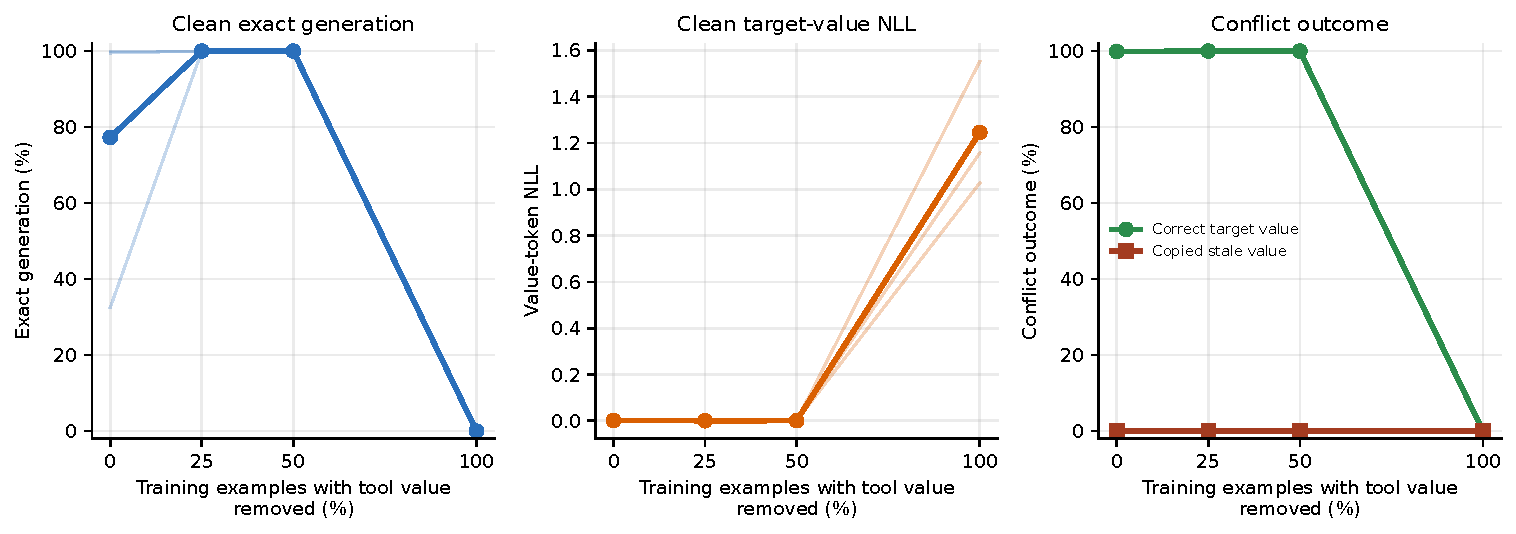
\includegraphics[width=\textwidth]{../figures/figure6_model_study.pdf}
\caption{
Controlled source-removal experiment across three optimization seeds.
(a) Clean exact generation. (b) Clean target-value negative log-likelihood.
(c) Conflict-set outcomes. Exact generation is 100\% at 25\% and 50\% source removal
and falls to zero when the tool value is removed from all training examples. In the
0\% condition, one seed frequently emits the correct value using \texttt{VALUE:}
instead of the prespecified \texttt{VALUE=} format, reducing its strict exact score
}
\label{fig:controlled}
\end{figure}

\begin{table}[ht]
\centering
\caption{
Controlled-model results, reported as mean $\pm$ optimization-seed SD across three seeds.
Exact generation requires the prespecified \texttt{VALUE=} field. NLL is computed over
target-value tokens.
}
\resizebox{\textwidth}{!}{\input{../tables/table4_model_study.tex}}
\end{table}

The unadapted model produces 0\% exact generation on both evaluation sets. With 0\%, 25\%,
50\%, and 100\% source removal during training, clean exact generation is 77.28\%, 100\%,
100\%, and 0\%, respectively. On the conflict set, the corresponding values are 99.89\%,
100\%, 100\%, and 0\%.

Complete source removal also increases target-value NLL from 0.000888 to 1.245163 on the clean
set and from 0.000776 to 1.039038 on the conflict set. For the 100\%-minus-0\% comparison,
paired-record 95\% bootstrap intervals are $[-78.56,-76.00]$ percentage points for clean exact
generation and $[1.2165,1.2710]$ for clean target-value NLL. The corresponding conflict intervals
are $[-100.00,-99.72]$ percentage points and $[1.0188,1.0597]$. These intervals resample
evaluation records while retaining all three trained seeds within each replicate; seed-level SD
is reported separately.
Table~9 reports the corresponding family-level results for the 0\% and 100\% source-removal conditions.

\begin{table}[ht]
\centering
\caption{
Family-level results for the 0\% and 100\% source-removal conditions. The lower strict clean
score at 0\% includes the output-format variation observed in one optimization seed.
}
\resizebox{\textwidth}{!}{\input{../tables/tableS2_model_families.tex}}
\end{table}

The lower clean exact score at 0\% source removal is largely a formatting effect. Seed 20260810
scores 195/600 under the strict parser because many correct values are emitted as
\texttt{VALUE:target}; the other two seeds score 599/600 and 597/600. On the conflict set, the
same three models score 599/600, 599/600, and 600/600. The low-scoring clean seed also retains
low target-value NLL.

As a format diagnostic, searching the generated text for the held-out value finds the correct
value in 99.39\% $\pm$ 0.67 of clean generations at 0\% source removal, 100\% at 25\% and
50\%, and 0\% at 100\%. No model copies the stale value on the conflict set.
\end{appendices}

\bibliography{references}
\end{document}
